\documentclass[11pt]{article}

\usepackage[margin=1in]{geometry}
\usepackage{amsmath,amssymb}
\usepackage{booktabs}
\usepackage{graphicx}
\usepackage{tikz}
\usetikzlibrary{arrows.meta,positioning,fit,backgrounds,calc}
\usepackage{algorithm}
\usepackage{algpseudocode}
\usepackage{siunitx}
\usepackage{caption}
\usepackage[hidelinks]{hyperref}

\sisetup{detect-weight=true}

\newcommand{\dispo}{\texttt{final\_disposition}}
\newcommand{\code}[1]{\texttt{#1}}

\title{\bfseries Predicting Supreme Court Case Outcomes\\ with a Bayesian Network:\\[0.3em]
\large A Baseline-Aware Evaluation}
\author{Matthew Park}
\date{July 28, 2026}

\begin{document}
\maketitle

\begin{abstract}
\noindent
The Supreme Court is one of the most powerful bodies in the United States
government, and knowing which way it would lean on a particular case has
obvious value. This paper builds a Bayesian network over the Supreme Court
Database and asks whether case outcomes can be predicted from case attributes.
The answer depends entirely on \emph{which} attributes are permitted. Using all
observable variables --- several of which are recorded from the decision itself
--- the network reaches \SI{81.7}{\percent} Top-3 accuracy, comfortably above a
no-features baseline at \SI{76.1}{\percent}. Restricted to information available
\emph{before} the Court rules, it reaches \SI{76.1}{\percent} Top-3: identical
to the baseline that ignores every feature, and slightly worse on log-loss.
We report proper scoring rules with bootstrap confidence intervals against four
reference models, diagnose the structural reason the pre-decision model fails,
and show that a BIC-scored structure search beats the hand-drawn graph on
held-out log-likelihood. The negative result is the substantive one: on this
feature set, most apparent predictive power is base rate.
\end{abstract}

\section{Introduction}

An earlier version of this work reported \SI{73}{\percent} Top-3 accuracy on 30
test cases and concluded that the network offered ``a clear increase in accuracy
than one could give on their own intuition.'' Both halves of that claim turned
out to be unsupported. A 30-case test set carries a bootstrap confidence
interval of roughly $\pm 16$ percentage points, and --- more importantly --- no
baseline was computed, so there was nothing to compare the number against.

The Court's dispositions are severely imbalanced. Across the full dataset,
\emph{affirmed} occurs in \SI{30.1}{\percent} of cases, \emph{reversed and
remanded} in \SI{27.5}{\percent}, and \emph{reversed} in \SI{22.0}{\percent}.
Those three outcomes alone account for \SI{79.6}{\percent} of all cases. A model
that ignores every feature and names those three every single time therefore
scores about \SI{80}{\percent} Top-3 --- above the figure the original write-up
presented as evidence that the model worked.

This paper rebuilds the model and, more consequentially, rebuilds its
evaluation. The contributions are:

\begin{enumerate}
  \item \textbf{Two evidence policies over one graph} (Section~\ref{sec:tracks}),
        separating a descriptive model that may use post-decision variables from
        a genuine forecast that may not.
  \item \textbf{Exact inference by variable elimination} (Section~\ref{sec:inference}),
        which both replaces sampling as the default and serves as ground truth
        for validating the three sampling engines.
  \item \textbf{Hierarchical backoff CPTs} (Section~\ref{sec:cpt}), addressing
        the finding that \SI{57.2}{\percent} of the parent configurations this
        network requires were never observed during training.
  \item \textbf{Baseline-anchored evaluation} (Section~\ref{sec:results}) with
        proper scoring rules and bootstrap confidence intervals against four
        reference models.
  \item \textbf{A structural diagnosis} (Section~\ref{sec:diagnosis}) of
        \emph{why} the pre-decision model cannot beat its baseline, and a
        structure search (Section~\ref{sec:structure}) showing the hand-drawn
        graph is not the best available.
\end{enumerate}

\section{Data}

We use the Supreme Court Database (SCDB) 2024\_01 case-centered release
\cite{scdb}, comprising 9{,}277 cases. After validation and removal of rows
lacking a recorded disposition, 9{,}141 cases are retained. We split
\textbf{chronologically}: the 7{,}312 earliest cases form the training set and
the 1{,}829 most recent form the test set. A chronological split matters here
because a random split would let the model train on future cases to predict past
ones, which no deployed forecaster could do.

\paragraph{A correction to the variable set.}
SCDB ships a column named \code{splitVote}, which reads naturally as ``the
justices were divided.'' It is not. It is an internal record-keeping flag
marking cases whose votes span multiple records, and it is \textbf{constant
($=1$) across all 9{,}277 rows}. A node fed by a constant carries no
information, and the earlier model included one. The pipeline now derives
\[
  \code{voteSplit} = \big(\code{minVotes} > 0\big),
\]
which splits 5{,}733 / 3{,}544 and does carry signal.

The 11 disposition codes are listed in Table~\ref{tab:dispositions}.

\begin{table}[t]
\centering
\caption{SCDB disposition codes, the 11-class prediction target.}
\label{tab:dispositions}
\footnotesize
\setlength{\tabcolsep}{4pt}
\begin{tabular}{cl@{\hskip 1em}cl}
\toprule
Code & Disposition & Code & Disposition \\
\midrule
1 & Stay, petition, or motion granted   & 7  & Affirmed and reversed in part and remanded \\
2 & Affirmed (includes modified)        & 8  & Vacated \\
3 & Reversed                            & 9  & Petition denied or appeal dismissed \\
4 & Reversed and remanded               & 10 & Certification to or from a lower court \\
5 & Vacated and remanded                & 11 & No disposition \\
6 & Affirmed and reversed in part       &    & \\
\bottomrule
\end{tabular}
\end{table}

\section{Network Structure}

The network is a four-layer directed acyclic graph over ten variables
(Figure~\ref{fig:dag}). Layer~1 carries court-level context; Layer~2 holds case
properties as root nodes; Layer~3 holds intermediate nodes that mediate between
case properties and the outcome; Layer~4 is the prediction target.

\begin{figure}[t]
\centering
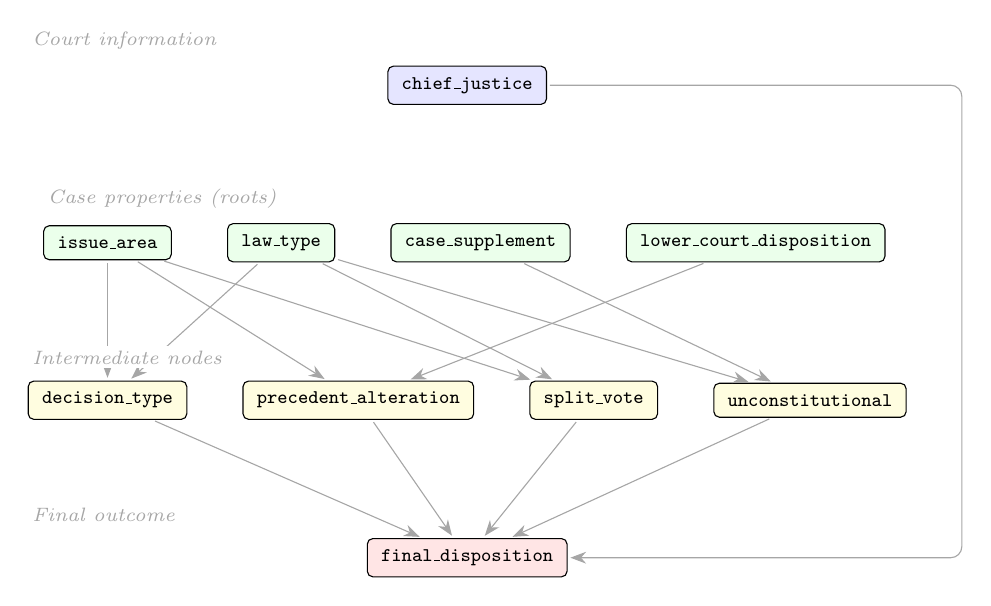
\begin{tikzpicture}[
  >={Stealth[length=2mm]},
  var/.style={draw, rounded corners=2pt, font=\scriptsize\ttfamily,
              inner xsep=5pt, inner ysep=4pt, align=center},
  root/.style={var, fill=green!8},
  midlayer/.style={var, fill=yellow!12},
  outcome/.style={var, fill=red!10},
  courtinfo/.style={var, fill=blue!10},
  lbl/.style={font=\scriptsize\itshape, gray!70, fill=white, inner sep=1.5pt},
  e/.style={->, gray!70, shorten >=1pt, shorten <=1pt}
]

% Layer 2 and 3 are chained with `right=of`, so TikZ derives the horizontal
% spacing from the actual typeset width of each label rather than an estimate.
\node[root] (issue) at (0,0) {issue\_area};
\node[root, right=7mm of issue] (law)  {law\_type};
\node[root, right=7mm of law]   (supp) {case\_supplement};
\node[root, right=7mm of supp]  (lcd)  {lower\_court\_disposition};

\node[midlayer] (dtype) at (0,-2) {decision\_type};
\node[midlayer, right=7mm of dtype] (prec)  {precedent\_alteration};
\node[midlayer, right=7mm of prec]  (split) {split\_vote};
\node[midlayer, right=7mm of split] (uncon) {unconstitutional};

% Chief justice and the outcome are centred on the widest row.
\node[courtinfo] at ($(dtype.west)!0.5!(uncon.east)+(0,4)$) (chief) {chief\_justice};
\node[outcome]   at ($(dtype.west)!0.5!(uncon.east)+(0,-2)$) (disp)  {final\_disposition};

\draw[e] (issue) -- (dtype);
\draw[e] (law)   -- (dtype);
\draw[e] (issue) -- (prec);
\draw[e] (lcd)   -- (prec);
\draw[e] (issue) -- (split);
\draw[e] (law)   -- (split);
\draw[e] (law)   -- (uncon);
\draw[e] (supp)  -- (uncon);

\draw[e] (dtype) -- (disp);
\draw[e] (prec)  -- (disp);
\draw[e] (split) -- (disp);
\draw[e] (uncon) -- (disp);

% chief_justice -> final_disposition is routed down the right-hand margin so it
% passes outside every other node instead of cutting through the middle layers.
\coordinate (rx) at ([xshift=7mm]uncon.east);
\draw[e, rounded corners=4pt]
  (chief.east) -- (chief.east -| rx) -- (disp.east -| rx) -- (disp.east);

% Layer captions sit on their own line above each row, clear of all nodes.
\node[lbl, anchor=south west] at ([yshift=1.5mm]chief.north  -| dtype.west) {Court information};
\node[lbl, anchor=south west] at ([yshift=1.5mm]issue.north  west) {Case properties (roots)};
\node[lbl, anchor=south west] at ([yshift=1.5mm]dtype.north  west) {Intermediate nodes};
\node[lbl, anchor=south west] at ([yshift=1.5mm]disp.north   -| dtype.west) {Final outcome};

\end{tikzpicture}
\caption{The hand-crafted network: 10 variables, 13 edges. Shading marks the
four layers. Note that every Layer-2 variable except \code{chief\_justice}
reaches the outcome \emph{only} through the intermediate layer --- the fact that
drives the result in Section~\ref{sec:diagnosis}.}
\label{fig:dag}
\end{figure}

\subsection{Two evidence policies over one graph}
\label{sec:tracks}

The same DAG supports two different experiments, distinguished only by which
variables are supplied as evidence at prediction time. The graph and the CPTs
are identical in both.

\begingroup\sloppy
\begin{description}
  \item[\code{explanatory}] All nine observable variables. Several of these ---
    \code{decision\_type}, \code{split\_vote}, \code{unconstitutional},
    \code{precedent\_alteration}, \code{case\_supplement} --- are recorded
    \emph{from} the decision and are simply not available beforehand. This track
    is a description of how case attributes co-occur with outcomes. It is not a
    forecast.
  \item[\code{ex\_ante}] Only the four variables knowable before the Court
    deliberates: \code{chief\_justice}, \code{issue\_area}, \code{law\_type},
    and \code{lower\_court\_disposition}. The intermediate nodes become
    unobserved, so the posterior must marginalise over them.
\end{description}
\endgroup

Keeping both tracks in the same codebase is deliberate. The gap between them is
the honest measure of how much of the explanatory track's performance comes from
peeking at the answer.

\section{Conditional Probability Tables}
\label{sec:cpt}

Root nodes use a Laplace-smoothed marginal with strength $\alpha$:
\[
  P(X = x) = \frac{N(X = x) + \alpha}{N + \alpha \lvert X \rvert}.
\]

Child nodes are the harder case. The naive estimator,
\[
  P\big(X = x \mid \mathrm{Pa}(X) = \mathbf{u}\big)
  = \frac{N(X = x, \mathrm{Pa}(X) = \mathbf{u})}{N(\mathrm{Pa}(X) = \mathbf{u})},
\]
is undefined whenever the parent configuration $\mathbf{u}$ never occurs in
training. This is not a rare edge case: \dispo{} has five parents, and
\textbf{\SI{57.2}{\percent} of the parent configurations the network needs were
never observed}. The earlier implementation answered every one of them with a
\emph{uniform} distribution --- the least informative guess available --- and
did so silently.

We instead use \textbf{hierarchical backoff} via Jelinek--Mercer interpolation.
Writing $\mathbf{u}_k$ for the first $k$ parents in a fixed ordering:
\begin{equation}
  P_k(x \mid \mathbf{u}_k)
  = \lambda_k \, P_{\mathrm{ML}}(x \mid \mathbf{u}_k)
  + (1 - \lambda_k) \, P_{k-1}(x \mid \mathbf{u}_{k-1}),
  \qquad
  \lambda_k = \frac{N(\mathbf{u}_k)}{N(\mathbf{u}_k) + m},
  \label{eq:backoff}
\end{equation}
with $P_0$ the smoothed marginal. A configuration observed far more than $m$
times is trusted almost entirely; a rare one is pulled toward an estimate
conditioning on fewer parents. Crucially, an unobserved configuration now falls
back to a genuinely informative lower-order estimate rather than to uniform. The
realised backoff rate is reported on every run rather than left implicit.

\section{Inference}
\label{sec:inference}

Four engines sit behind a single \code{query} interface.

\subsection{Exact inference}

Variable elimination computes the posterior exactly by summing out non-evidence,
non-query variables in turn:
\[
  P(\dispo \mid \mathbf{e}) \;\propto\;
  \sum_{\mathbf{h}} \prod_{i} P\big(X_i \mid \mathrm{Pa}(X_i)\big),
\]
where $\mathbf{h}$ ranges over hidden variables. With ten variables and modest
cardinalities this is trivially cheap, and it is exact.

\subsection{Sampling engines and their validation}

The three sampling engines --- rejection sampling, likelihood weighting, and
Gibbs (MCMC) --- are retained, but their role has changed. Previously they could
only be compared to \emph{one another}, which cannot distinguish ``all three are
correct'' from ``all three share a bug.'' With an exact posterior available,
each can be validated against a known answer.

\begin{algorithm}[t]
\caption{Rejection sampling (retained for comparison)}
\begin{algorithmic}[1]
\Require CPTs, observations $\mathbf{e}$, target value $y$, sample budget $N$
\Ensure Estimate of $P(\dispo = y \mid \mathbf{e})$
\State $\textit{hits} \gets 0$; \quad $\textit{accepted} \gets 0$
\For{$i = 1$ \textbf{to} $N$}
  \State $s \gets \Call{AncestralSample}{\text{CPTs}}$
  \If{$s$ agrees with $\mathbf{e}$ on every observed variable}
    \State $\textit{accepted} \gets \textit{accepted} + 1$
    \If{$s[\dispo] = y$} $\textit{hits} \gets \textit{hits} + 1$ \EndIf
  \EndIf
\EndFor
\State \Return $\textit{accepted} = 0$ \textbf{?} $0$ \textbf{:} $\textit{hits}/\textit{accepted}$
\end{algorithmic}
\end{algorithm}

Table~\ref{tab:engines} gives accuracy, wall-clock time, and total-variation
distance from the exact posterior on the explanatory track.

\begin{table}[t]
\centering
\caption{Inference engines on the explanatory track (200 test cases).}
\label{tab:engines}
\begin{tabular}{lrrr}
\toprule
Engine & Top-3 & Time & TV distance from exact \\
\midrule
Exact (variable elimination) & \textbf{87.0\%} & \textbf{0.02 s} & --- (reference) \\
Rejection sampling           & 55.5\% & 28.56 s & 0.5477 \\
Likelihood weighting         & 87.0\% & 8.27 s  & 0.0257 \\
Gibbs sampling (MCMC)        & 87.0\% & 13.38 s & 0.0232 \\
\bottomrule
\end{tabular}
\end{table}

Rejection sampling's collapse is the textbook failure mode, now measured rather
than asserted: with nine evidence variables almost every sample is discarded,
leaving the estimate both wrong (TV $0.55$) and $1400\times$ slower than exact.
Table~\ref{tab:convergence} shows the two weighted samplers converging toward the
exact posterior as the budget grows. Rejection sampling does not converge cleanly,
and its row is not reproducible between runs.

\begin{table}[t]
\centering
\caption{Total-variation distance from the exact posterior versus sample budget.
Likelihood weighting and Gibbs reproduce exactly on every run; the rejection
sampling row is one observed run of many possible ones (see text).}
\label{tab:convergence}
\begin{tabular}{lrrrr}
\toprule
Engine & 100 & 500 & 1000 & 5000 \\
\midrule
Rejection sampling$^{\dagger}$ & 0.5486 & 0.2546 & 0.1514 & 0.2276 \\
Likelihood weighting & 0.1134 & 0.0354 & 0.0164 & 0.0132 \\
Gibbs sampling       & 0.1045 & 0.0376 & 0.0226 & 0.0136 \\
\bottomrule
\end{tabular}
\end{table}

\paragraph{$^{\dagger}$ On the irreproducibility of the rejection row.}
Repeated invocations at a fixed seed have produced
$0.5486 / 0.8192 / 0.8192 / 0.1514$ and $0.5486 / 0.5486 / 0.9087 / 0.2269$
alongside the row above, and the sequence is not monotone in the sample budget.
The cause is not sampling noise in the ordinary sense. \code{CPTBuilder.get\_values}
returns a \code{set}, so nodes taking string values iterate in an order that
Python's per-process hash randomisation varies from run to run; the index a given
random draw selects therefore maps to a different value each time. Likelihood
weighting and Gibbs are insensitive to this because they aggregate over every
value of a node. Rejection sampling, accepting on the order of one sample in a
hundred under nine evidence variables, rests on so few accepted draws that the
ordering determines the estimate. Sorting the value sets would restore
determinism at the cost of remapping every sampler's draws, and with them the
figures reported elsewhere in this paper; the instability is recorded here
rather than papered over.

Exact inference is also the right default for a further reason: when all of a
leaf's parents are observed, the posterior is a single CPT row. The sampling
engines were spending 1{,}000 draws to approximate a dictionary lookup.

\section{Evaluation Methodology}

\paragraph{Reference models.}
Four baselines implement the same \code{query} interface as the network and run
through the identical evaluation path: a \textbf{marginal} model that ignores
all features and returns the training base rate; a \textbf{majority-class}
model; \textbf{multinomial logistic regression}; and \textbf{gradient boosting}.
The marginal model is the one that matters --- it is the floor any claim of
predictive power must clear.

\paragraph{Metrics.}
We report Top-$k$ accuracy for $k \in \{1,3,5\}$ alongside \textbf{proper
scoring rules}: log-loss, Brier score, expected calibration error, and macro
one-vs-rest AUC. Proper scoring rules cannot be gamed by predicting the marginal
distribution, which on this task is precisely the failure mode worth guarding
against. Every point estimate carries a bootstrap \SI{95}{\percent} confidence
interval over 500 resamples.

\section{Results}
\label{sec:results}

\begin{table}[t]
\centering
\caption{Multi-class disposition (11 classes), \textbf{explanatory} track ---
all observable variables, including several recorded from the decision.
Brackets are bootstrap \SI{95}{\percent} CIs.}
\label{tab:explanatory}
\footnotesize
\setlength{\tabcolsep}{4pt}
\begin{tabular}{lccccccc}
\toprule
Model & Top-1 & Top-3 & Top-5 & Log-loss & Brier & ECE & AUC \\
\midrule
Marginal (no features) & 26.7 [24.4, 28.6] & 76.1 [74.5, 77.9] & 97.1 & 1.6244 & 0.7777 & 0.042 & 0.500 \\
Majority class         & 26.7 [24.4, 28.6] & 39.3 [37.1, 41.6] & 94.8 & 5.0015 & 1.4502 & 0.723 & 0.500 \\
Logistic regression    & \textbf{34.2} [32.0, 36.3] & 81.4 [79.7, 83.0] & \textbf{98.3} & \textbf{1.5302} & \textbf{0.7474} & 0.044 & \textbf{0.718} \\
Gradient boosting      & 33.6 [31.6, 35.5] & 80.5 [78.8, 82.1] & 97.9 & 1.6187 & 0.7593 & 0.095 & 0.658 \\
\textbf{Bayesian network} & 32.6 [30.4, 34.5] & \textbf{81.7} [80.0, 83.4] & 98.0 & 1.5920 & 0.7495 & 0.050 & 0.553 \\
\bottomrule
\end{tabular}
\end{table}

\begin{table}[t]
\centering
\caption{Multi-class disposition (11 classes), \textbf{ex-ante} track --- only
information knowable before the Court rules.}
\label{tab:exante}
\footnotesize
\setlength{\tabcolsep}{4pt}
\begin{tabular}{lccccccc}
\toprule
Model & Top-1 & Top-3 & Top-5 & Log-loss & Brier & ECE & AUC \\
\midrule
Marginal (no features) & 26.7 [24.4, 28.6] & 76.1 [74.5, 77.9] & 97.1 & \textbf{1.6244} & 0.7777 & 0.042 & 0.500 \\
Logistic regression    & 29.4 [27.3, 31.2] & 77.9 [76.2, 79.6] & \textbf{97.9} & 1.6116 & \textbf{0.7749} & 0.077 & \textbf{0.673} \\
Gradient boosting      & \textbf{30.2} [28.2, 32.5] & \textbf{78.5} [76.8, 80.0] & 97.2 & 1.6901 & 0.7822 & 0.090 & 0.659 \\
\textbf{Bayesian network} & 27.0 [24.7, 29.0] & 76.1 [74.5, 77.9] & 97.8 & 1.6339 & 0.7764 & 0.064 & 0.520 \\
\bottomrule
\end{tabular}
\end{table}

Table~\ref{tab:explanatory} shows the network at \SI{81.7}{\percent} Top-3,
above the no-features baseline at \SI{76.1}{\percent} with non-overlapping
confidence intervals. That is a real effect. It is also not a forecast: five of
the nine evidence variables are recorded from the decision being predicted.

Table~\ref{tab:exante} is the honest headline. Restricted to pre-decision
information, the network scores \SI{76.1}{\percent} Top-3 --- \emph{identical}
to the model that ignores every feature --- and is slightly \emph{worse} on
log-loss (1.6339 versus 1.6244). The two tree-based reference models do
marginally better, but neither clears its baseline by more than the interval
width.

\subsection{Binary affirm / reverse}

Table~\ref{tab:binary} reports the standard formulation in the literature:
affirm $=$ disposition~2, reverse/vacate $=$ dispositions 3, 4, 5, 8, other
dispositions excluded ($n = 1{,}729$).

\begin{table}[t]
\centering
\caption{Binary affirm / reverse task ($n = 1{,}729$).}
\label{tab:binary}
\begin{tabular}{llccc}
\toprule
Model & Track & Accuracy & Log-loss & AUC \\
\midrule
Marginal (no features) & ---          & 71.8 [69.6, 73.7] & 0.6015 & 0.500 \\
Bayesian network       & explanatory  & \textbf{72.6} [70.4, 74.7] & \textbf{0.5703} & 0.599 \\
Logistic regression    & explanatory  & 72.1 [69.7, 74.1] & 0.5644 & \textbf{0.663} \\
Bayesian network       & ex\_ante     & 71.8 [69.6, 73.7] & 0.6036 & 0.561 \\
Gradient boosting      & ex\_ante     & 69.7 [67.5, 71.7] & 0.6042 & 0.572 \\
\bottomrule
\end{tabular}
\end{table}

Katz, Bommarito \& Blackman \cite{katz2017} report roughly \SI{70.2}{\percent}
case-level accuracy on this task using time-evolving random forests over a much
larger feature set and a different evaluation protocol; the numbers are not
directly comparable. The more useful observation is that \emph{always predicting
``reversed''} scores \SI{71.8}{\percent} on this test set, because the Court
reverses far more often than it affirms. Any binary accuracy figure in this
literature --- including ours --- should be read against that floor.

\subsection{What the AUC column says}

AUC exceeds 0.5 everywhere, including the ex-ante track (0.520--0.673). There
\emph{is} signal in pre-decision variables: the models rank cases better than
chance. It is simply not enough to change which class ends up on top, because
one class dominates. Reporting accuracy alone would conceal this; reporting AUC
and log-loss alongside it does not.

\section{Why the Ex-Ante Model Fails: A Structural Diagnosis}
\label{sec:diagnosis}

The ex-ante result is not a bug, and the graph explains it precisely. Of the
four pre-decision variables, only \code{chief\_justice} is a direct parent of
the outcome (Table~\ref{tab:bottleneck}).

\begin{table}[t]
\centering
\caption{Paths from ex-ante variables to the outcome. ``Direct parent?'' means a
direct parent of \dispo{} in the graph.}
\label{tab:bottleneck}
\footnotesize
\setlength{\tabcolsep}{5pt}
\begin{tabular}{llp{0.46\textwidth}}
\toprule
Ex-ante variable & Direct parent? & Reaches the outcome via \\
\midrule
\code{chief\_justice}            & yes & --- \\
\code{issue\_area}               & no  & \code{decision\_type}, \code{precedent\_alteration}, \code{split\_vote} \\
\code{law\_type}                 & no  & \code{decision\_type}, \code{split\_vote}, \code{unconstitutional} \\
\code{lower\_court\_disposition} & no  & \code{precedent\_alteration} only \\
\bottomrule
\end{tabular}
\end{table}

Every other ex-ante variable reaches \dispo{} \emph{only} through the four
intermediate nodes --- and all four are post-decision. When they are unobserved,
they act as a bottleneck that washes the signal out.

\code{lower\_court\_disposition} is the sharpest case. Whether the court below
affirmed or reversed is plausibly the single most informative thing knowable
before the ruling, and it is genuinely associated with the outcome in the data
($G = 352.4$, $\mathrm{df} = 99$, $p \approx 4 \times 10^{-30}$). But its only
path to the outcome runs through \code{precedent\_alteration}, a near-constant
binary. Conditioning on it moves the posterior by a total-variation distance of
approximately $0.001$. \emph{The information is present in the data and the
graph cannot carry it.}

This is pinned by a regression test, so that anyone who later adds a direct edge
will see the expectation fail and learn why it was there.

\section{Hand-Crafted versus Learned Structure}
\label{sec:structure}

If the intermediate layer is the problem, the natural question is whether the
data supports it at all. We ran BIC-scored hill-climbing from the empty graph
with add, remove, and reverse moves, and an in-degree cap of four
(Table~\ref{tab:structure}).

\begin{table}[t]
\centering
\caption{Hand-crafted versus learned network structure.}
\label{tab:structure}
\begin{tabular}{lrrr}
\toprule
 & BIC & Held-out log-likelihood & Edges \\
\midrule
Hand-crafted (domain) & $-82{,}533.75$ & $-15{,}088.07$ & 13 \\
Learned (BIC search)  & $\mathbf{-56{,}830.93}$ & $\mathbf{-14{,}315.70}$ & 11 \\
\bottomrule
\end{tabular}
\end{table}

The learned graph wins on BIC --- which it was optimising, so that is expected
--- but it also wins on \textbf{held-out log-likelihood}, which it was not. The
two graphs share only \textbf{3 of 13 edges}. The search adds
$\code{lawType} \rightarrow \code{caseDisposition}$ and drops most of the
hand-specified parents of the outcome, including \code{decisionType},
\code{chief}, \code{precedentAlteration}, and \code{declarationUncon}.

Read plainly: on this dataset the domain-informed structure is worse than one
derived from the data, and the intermediate-node layer is largely not earning
its place. This corroborates Section~\ref{sec:diagnosis} from an independent
direction.

We also replaced raw mutual information with \textbf{normalised} mutual
information and a $G$-test with proper degrees of freedom, since raw MI's
cardinality bias systematically favours high-arity variables in exactly the
pairwise screening the original structure was built from.

\section{Limitations}

\begin{itemize}
  \item \textbf{The ex-ante feature set is thin.} SCDB carries other genuinely
    pre-decision fields --- \code{certReason}, \code{jurisdiction},
    \code{lcDisagreement}, \code{caseSource} --- that are absent from the graph
    and would be the natural next extension. The negative result in
    Table~\ref{tab:exante} bounds \emph{this} feature set, not pre-decision
    prediction in general.
  \item \textbf{The intermediate layer is unsupported.} Structure search does
    not recover it, and the outcome node's five-parent family is sparse enough
    that \SI{57.2}{\percent} of its configurations require backoff.
  \item \textbf{Case-level modelling only.} The literature's stronger results
    come from justice-level vote prediction aggregated to a case outcome, which
    SCDB's justice-centered release supports and this work does not use.
\end{itemize}

\section{Conclusion}

A Bayesian network can describe the Supreme Court's record well: given all
observable case attributes, it reaches \SI{81.7}{\percent} Top-3 accuracy,
significantly above a no-features baseline. But most of those attributes are
recorded from the decision. Restricted to what is knowable beforehand, the same
network matches the baseline that ignores every feature and loses to it on
log-loss --- and the graph structure explains precisely why, with the most
informative pre-decision variable bottlenecked behind a near-constant
intermediate node.

The methodological point generalises beyond this dataset. On a task with an
\SI{80}{\percent} base rate concentrated in three classes, a Top-3 accuracy
figure reported without a baseline is uninterpretable, and one computed on 30
test cases is noise. The first version of this work reported exactly that. The
apparatus here --- baselines sharing the evaluation path, proper scoring rules,
bootstrap intervals, and an exact engine to validate the approximate ones ---
exists to make that particular mistake hard to repeat.

\begin{thebibliography}{9}
\bibitem{scdb}
Washington University Law. (2024). \emph{The Supreme Court Database},
2024\_01 case-centered release. \url{http://scdb.wustl.edu}

\bibitem{katz2017}
Katz, D. M., Bommarito, M. J., \& Blackman, J. (2017). A general approach for
predicting the behavior of the Supreme Court of the United States.
\emph{PLoS ONE}, 12(4), e0174698.

\bibitem{aima}
Russell, S., \& Norvig, P. \emph{Artificial Intelligence: A Modern Approach},
Ch.~14: Probabilistic reasoning and sampling methods for Bayesian networks.

\bibitem{koller}
Koller, D., \& Friedman, N. (2009). \emph{Probabilistic Graphical Models:
Principles and Techniques}. MIT Press.
\end{thebibliography}

\end{document}
